% Options for packages loaded elsewhere
\PassOptionsToPackage{unicode}{hyperref}
\PassOptionsToPackage{hyphens}{url}
%
\documentclass[
]{book}
\usepackage{amsmath,amssymb}
\usepackage{lmodern}
\usepackage{iftex}
\ifPDFTeX
  \usepackage[T1]{fontenc}
  \usepackage[utf8]{inputenc}
  \usepackage{textcomp} % provide euro and other symbols
\else % if luatex or xetex
  \usepackage{unicode-math}
  \defaultfontfeatures{Scale=MatchLowercase}
  \defaultfontfeatures[\rmfamily]{Ligatures=TeX,Scale=1}
\fi
% Use upquote if available, for straight quotes in verbatim environments
\IfFileExists{upquote.sty}{\usepackage{upquote}}{}
\IfFileExists{microtype.sty}{% use microtype if available
  \usepackage[]{microtype}
  \UseMicrotypeSet[protrusion]{basicmath} % disable protrusion for tt fonts
}{}
\makeatletter
\@ifundefined{KOMAClassName}{% if non-KOMA class
  \IfFileExists{parskip.sty}{%
    \usepackage{parskip}
  }{% else
    \setlength{\parindent}{0pt}
    \setlength{\parskip}{6pt plus 2pt minus 1pt}}
}{% if KOMA class
  \KOMAoptions{parskip=half}}
\makeatother
\usepackage{xcolor}
\usepackage{longtable,booktabs,array}
\usepackage{calc} % for calculating minipage widths
% Correct order of tables after \paragraph or \subparagraph
\usepackage{etoolbox}
\makeatletter
\patchcmd\longtable{\par}{\if@noskipsec\mbox{}\fi\par}{}{}
\makeatother
% Allow footnotes in longtable head/foot
\IfFileExists{footnotehyper.sty}{\usepackage{footnotehyper}}{\usepackage{footnote}}
\makesavenoteenv{longtable}
\usepackage{graphicx}
\makeatletter
\def\maxwidth{\ifdim\Gin@nat@width>\linewidth\linewidth\else\Gin@nat@width\fi}
\def\maxheight{\ifdim\Gin@nat@height>\textheight\textheight\else\Gin@nat@height\fi}
\makeatother
% Scale images if necessary, so that they will not overflow the page
% margins by default, and it is still possible to overwrite the defaults
% using explicit options in \includegraphics[width, height, ...]{}
\setkeys{Gin}{width=\maxwidth,height=\maxheight,keepaspectratio}
% Set default figure placement to htbp
\makeatletter
\def\fps@figure{htbp}
\makeatother
\setlength{\emergencystretch}{3em} % prevent overfull lines
\providecommand{\tightlist}{%
  \setlength{\itemsep}{0pt}\setlength{\parskip}{0pt}}
\setcounter{secnumdepth}{5}
\ifLuaTeX
\usepackage[bidi=basic]{babel}
\else
\usepackage[bidi=default]{babel}
\fi
\babelprovide[main,import]{brazilian}
% get rid of language-specific shorthands (see #6817):
\let\LanguageShortHands\languageshorthands
\def\languageshorthands#1{}
\usepackage{booktabs}
\ifLuaTeX
  \usepackage{selnolig}  % disable illegal ligatures
\fi
\usepackage[]{natbib}
\bibliographystyle{plainnat}
\IfFileExists{bookmark.sty}{\usepackage{bookmark}}{\usepackage{hyperref}}
\IfFileExists{xurl.sty}{\usepackage{xurl}}{} % add URL line breaks if available
\urlstyle{same} % disable monospaced font for URLs
\hypersetup{
  pdftitle={Bookdown Resumo dos Slides},
  pdfauthor={Daniel Claudino},
  pdflang={pt-BR},
  hidelinks,
  pdfcreator={LaTeX via pandoc}}

\title{Bookdown Resumo dos Slides}
\author{Daniel Claudino}
\date{2022-11-01}

\begin{document}
\maketitle

{
\setcounter{tocdepth}{1}
\tableofcontents
}
\hypertarget{apresentauxe7uxe3o}{%
\chapter{Apresentação}\label{apresentauxe7uxe3o}}

Bookdown Resumo dos Slides das Disciplinas

\begin{figure}

{\centering 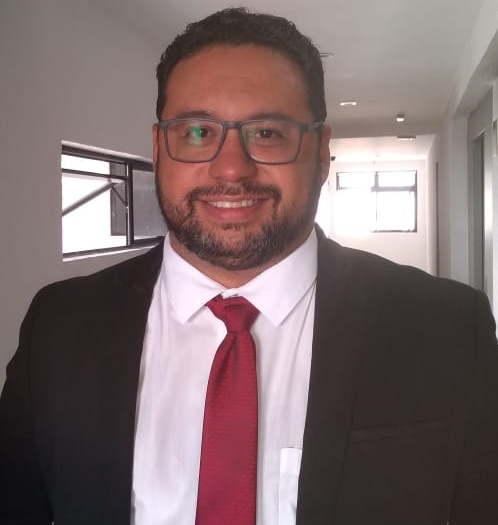
\includegraphics[width=0.5\linewidth]{imagens/FOTO-PERFIL-DANIEL-CLAUDINO-2020} 

}

\caption{Autor: Daniel Claudino}\label{fig:unnamed-chunk-1}
\end{figure}

Neste bookdown estarão conditos os resumos dos slides das disciplinas do 1º até o 10º período do curso de Bacharelado em Psicologia.

\hypertarget{controle-de-versuxe3o}{%
\section{Controle de Versão}\label{controle-de-versuxe3o}}

\begin{longtable}[]{@{}
  >{\raggedright\arraybackslash}p{(\columnwidth - 6\tabcolsep) * \real{0.2500}}
  >{\raggedright\arraybackslash}p{(\columnwidth - 6\tabcolsep) * \real{0.2500}}
  >{\raggedright\arraybackslash}p{(\columnwidth - 6\tabcolsep) * \real{0.2500}}
  >{\raggedright\arraybackslash}p{(\columnwidth - 6\tabcolsep) * \real{0.2500}}@{}}
\toprule()
\begin{minipage}[b]{\linewidth}\raggedright
Versão
\end{minipage} & \begin{minipage}[b]{\linewidth}\raggedright
Data / Hora
\end{minipage} & \begin{minipage}[b]{\linewidth}\raggedright
Colaborador
\end{minipage} & \begin{minipage}[b]{\linewidth}\raggedright
Descrição da Contribuição
\end{minipage} \\
\midrule()
\endhead
0.1 & 01/11/2022 09h41 & \href{https://wa.me/5583988853815}{Daniel Claudino} & Versão inicial do documento \\
\bottomrule()
\end{longtable}

\hypertarget{referuxeancias-bibliogruxe1ficas}{%
\section{Referências Bibliográficas}\label{referuxeancias-bibliogruxe1ficas}}

\hypertarget{bibliografia-buxe1sica}{%
\subsection{Bibliografia Básica}\label{bibliografia-buxe1sica}}

DAVIDOFF, Linda L. Introdução à Psicologia. São Paulo: Makron Books, 2001.

SPINK, M. J. P. Psicologia social e saúde: práticas, saberes e sentidos. Petrópolis:Vozes, 2013.

MAISTO, Albert A.; MORRIS, Charles G. Introdução a Psicologia. 6 ed.~São Paulo, Prentice Hall, 2004. {[}Livro Eletrônico{]}

\hypertarget{bibliografia-complementar}{%
\subsection{Bibliografia Complementar}\label{bibliografia-complementar}}

BRIGAGÃO, J., NASCIMENTO, V. L. V., \& SPINK, P. K. (2011). As interfaces entre psicologia e políticas públicas e a configuração de novos espaços de atuação. Sorocaba, (páginas, 199-215).

CASTRO, E. K., \& BORNHOLDT, E. (2004). Psicologia da saúde x psicologia hospitalar: definições e possibilidades de inserção profissional. Psicologia Ciência e Profissão (páginas, 48-57).

COELHO, Wilson Ferreira. Psicologia do Desenvolvimento. São Paulo: Editora Pearson, 2014. {[}Livro Eletrônico{]}

CÓRIA-SABINI, Maria Aparecida. Psicologia do Desenvolvimento. 2 ed.~São Paulo: Editora Ática, 2010. {[}Livro Eletrônico{]}

DIAS, A. C. G., PATIAS, N. D., \& ABAID, J. L. W. ( 2014). Psicologia escolar e possibilidades na atuação do psicólogo: algumas reflexões. Revista Psicologia Escolar e Educacional (páginas 105-111).

FEIST, J., FEIST, G., \& ROBERTS, T. A. (2015). Teorias da Personalidade.

FELDMAN, Robert S. Introdução à Psicologia. Porto Alegre: Editora AMGH,2015.

ILETTI, Nelson; ROSSATO, Solange Marques; ROSSATO, Geovanio. Psicologia do Desenvolvimento. São Paulo, Contexto, 2014. {[}Livro Eletrônico{]}

LIMA, C. F., \& PIMENTEL, C. E. (2017). Livro: Revisitando a Psicologia Social. MISKOLCI, Richard. Teoria Queer: um aprendizado pelas diferenças. 2 ed.~Belo Horizonte: Autêntica, 2015. {[}Livro Eletrônico{]}

PADILHA, S., NORONHA, A. P. P., \& ZANCHET, C. F. (2007). Instrumentos de avaliação psicológica: uso e parecer de psicólogos. Avaliação psicológica (páginas, 69-79).

SCHULTZ, D. \& SCHULTZ, S. E. (2019). História da Psicologia moderna.

ZANELLI, J. C., BASTOS, A. V. B., \& RODRIGUES, A. C. A. ( 2014). Psicologia, Organizações e Trabalho no Brasil. (Orgs).

\hypertarget{observauxe7uxe3o-importante}{%
\section{Observação Importante}\label{observauxe7uxe3o-importante}}

\textbf{NOTA}: Este material tem como finalidade auxiliar a fixação de assuntos estudados em sala de aula de acordo com o \textbf{plano de ensino desta disciplina}.

Ele \textbf{não deve ser} utilizado como \textbf{único material de estudo para a prova}, então:

\begin{enumerate}
\def\labelenumi{\arabic{enumi}.}
\tightlist
\item
  Consulte os \textbf{slides da professora} na plataforma FTM;\\
\item
  Faça \textbf{notas de aula} do que for tratado em sala de aula;\\
\item
  Consulte nossas \textbf{notas de aula};
\end{enumerate}

\begin{quote}
\textbf{Dúvidas}: Devem ser encaminhadas no grupo de whatsapp da disciplina.
\end{quote}

\hypertarget{p1---anatomia-humana}{%
\chapter{P1 - Anatomia Humana}\label{p1---anatomia-humana}}

Neste capítulo estarão contidos os resumos dos slides da disciplina Anatomia Humana. De acordo com o plano da disciplina, a professora adotou notas de aula como recurso didático, portanto não há resumos de slides a serem disponibilizados aqui.

\hypertarget{p1---introduuxe7uxe3o-uxe0-psicologia}{%
\chapter{P1 - Introdução à Psicologia}\label{p1---introduuxe7uxe3o-uxe0-psicologia}}

Neste capítulo estarão contidos os resumos dos slides da disciplina Introdução à Psicologia.

\hypertarget{slide-introduuxe7uxe3o-uxe0-psicologia}{%
\section{Slide ``Introdução à Psicologia''}\label{slide-introduuxe7uxe3o-uxe0-psicologia}}

\hypertarget{definiuxe7uxe3o-de-psicologia}{%
\subsection{Definição de Psicologia}\label{definiuxe7uxe3o-de-psicologia}}

\begin{itemize}
\tightlist
\item
  A palavra psicologia, deriva se da junção de dois termos gregos \emph{psiché} e \emph{logos} estudo da mente ou da alma''.
\item
  É a ciência que se concentra no comportamento e nos processos mentais
\end{itemize}

\hypertarget{definiuxe7uxe3o-de-construto}{%
\subsection{Definição de Construto}\label{definiuxe7uxe3o-de-construto}}

\begin{itemize}
\tightlist
\item
  Segundo Cronbach e Meehl(1955) e Primi(2018), um construto é:

  \begin{itemize}
  \tightlist
  \item
    Um atributo das pessoas;
  \item
    Não observável diretamente;
  \item
    Que se postula existir ;
  \item
    Que se assume estar refletido nos \textbf{comportamentos observados} \textbf{na testagem};
  \end{itemize}
\item
  Assim, é um \textbf{conceito teórico} sobre um \textbf{atributo latente} que \textbf{explica os comportamentos} na \textbf{testagem}.
\end{itemize}

\hypertarget{focalizando-o-geral}{%
\subsection{Focalizando o geral}\label{focalizando-o-geral}}

\begin{itemize}
\tightlist
\item
  Como cientistas

  \begin{itemize}
  \tightlist
  \item
    Os psicólogos estão rotineiramente tentando descobrir os princípios universais a partir de observações específicas que despertam a sua curiosidade;
  \end{itemize}
\end{itemize}

\hypertarget{a-psicologia-hoje}{%
\subsection{A Psicologia hoje}\label{a-psicologia-hoje}}

\begin{itemize}
\tightlist
\item
  Por sua definição, entende se a psicologia como uma disciplina única;
\item
  Cada uma das subáreas em que se divide a Psicologia tem \textbf{características} e \textbf{exigências} \textbf{próprias} e \textbf{exclusivas}.
\end{itemize}

\begin{longtable}[]{@{}
  >{\raggedright\arraybackslash}p{(\columnwidth - 2\tabcolsep) * \real{0.3478}}
  >{\raggedright\arraybackslash}p{(\columnwidth - 2\tabcolsep) * \real{0.6522}}@{}}
\toprule()
\begin{minipage}[b]{\linewidth}\raggedright
Subárea
\end{minipage} & \begin{minipage}[b]{\linewidth}\raggedright
Descrição
\end{minipage} \\
\midrule()
\endhead
Genética comportamental & A genética comportamental estuda a herança de traços relacionados ao comportamento. \\
Neurociência comportamental & A neurociência comportamental examina as bases biológicas do comportamento. \\
Psicologia clínica & A psicologia clínica trata do estudo, do diagnóstico e do tratamento de transtornos psicológicos. \\
Neuropsicologia clínica & A neuropsicologia clínica une as áreas da biopsicologia e da psicologia clínica, focando a relação entre fatores biológicos e transtornos psicológicos. \\
Psicologia cognitiva & A psicologia cognitiva centra-se no estudo dos processos mentais superiores. \\
Psicólogo de aconselhamento & O aconselhamento psicológico aborda principalmente problemas educacionais, sociais e de adaptação profissional. \\
Psicologia transcultural & A psicologia intercultural investiga as semelhanças e diferenças no funcionamento psicológico nas várias culturas e nos grupos étnicos. \\
Psicologia do desenvolvimento & A psicologia do desenvolvimento examina como as pessoas crescem e mudam a partir do momento da concepção até a morte. \\
Psicologia educacional & A psicologia educacional ocupa-se do ensino e dos processos aprendizagem, tais como a relação entre motivação e desempenho na escola. \\
Psicologia ambiental & A psicologia ambiental considera a relação entre as pessoas e o ambiente físico. \\
Psicologia evolucionista & A psicologia evolucionista considera como o comportamento é influenciado pela herança genética de nossos antepassados. \\
Psicologia experimental & A psicologia experimental estuda os processos de sentir, perceber, aprender e pensar sobre o mundo. \\
Psicologia forense & A psicologia forense aborda questões legais, tais como determinar a precisão das memórias de testemunhas. \\
Psicologia da saúde & A psicologia da saúde explora a relação entre fatores psicológicos e enfermidades físicas, ou doenças. \\
Psicologia industrial/organizacional & A psicologia industrial/organizacional preocupa-se com a psicologia do local de trabalho. \\
Psicologia da personalidade & A psicologia da personalidade analisa a consistência no comportamento das pessoas ao longo do tempo e as características que diferenciam uma pessoa da outra. \\
Psicologia das mulheres & A psicologia das mulheres aborda questões como a discriminação contra mulheres e as causas da violência contra mulheres. \\
Psicologia escolar & A psicologia escolar é dedicada ao aconselhamento de crianças que têm problemas acadêmicos ou emocionais nas escolas primárias e secundárias. \\
Psicologia social & A psicologia social é o estudo de como os pensamentos, os sentimentos e as ações das pessoas são afetadas pelos outros. \\
Psicologia do esporte & A psicologia do esporte aplica a psicologia à atividade e ao exercício esportivo. \\
\bottomrule()
\end{longtable}

\begin{quote}
****QUESTÃO DE PROVA****: Cite 03 subáreas da psicologia e sua atuação
\end{quote}

\begin{figure}

{\centering 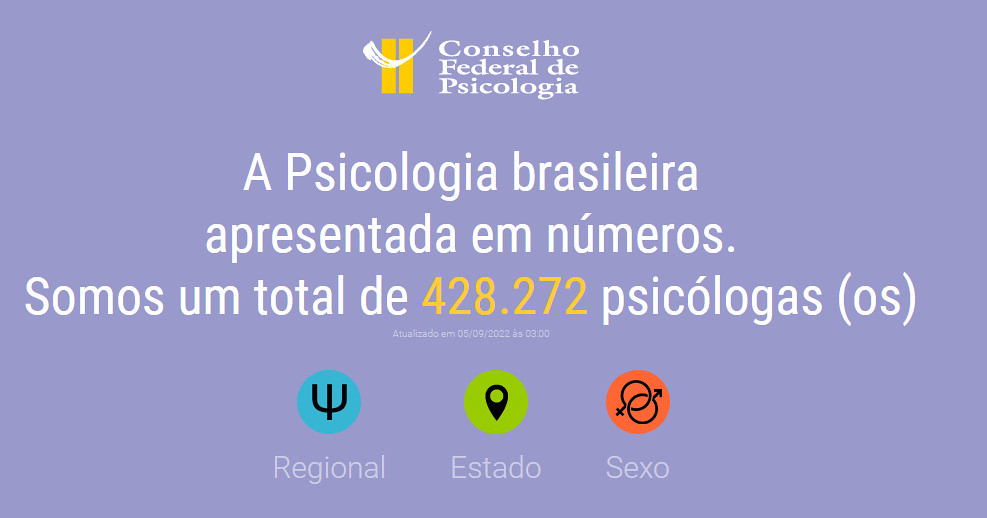
\includegraphics[width=0.5\linewidth]{imagens/numero-de-psicologos-no-brasil} 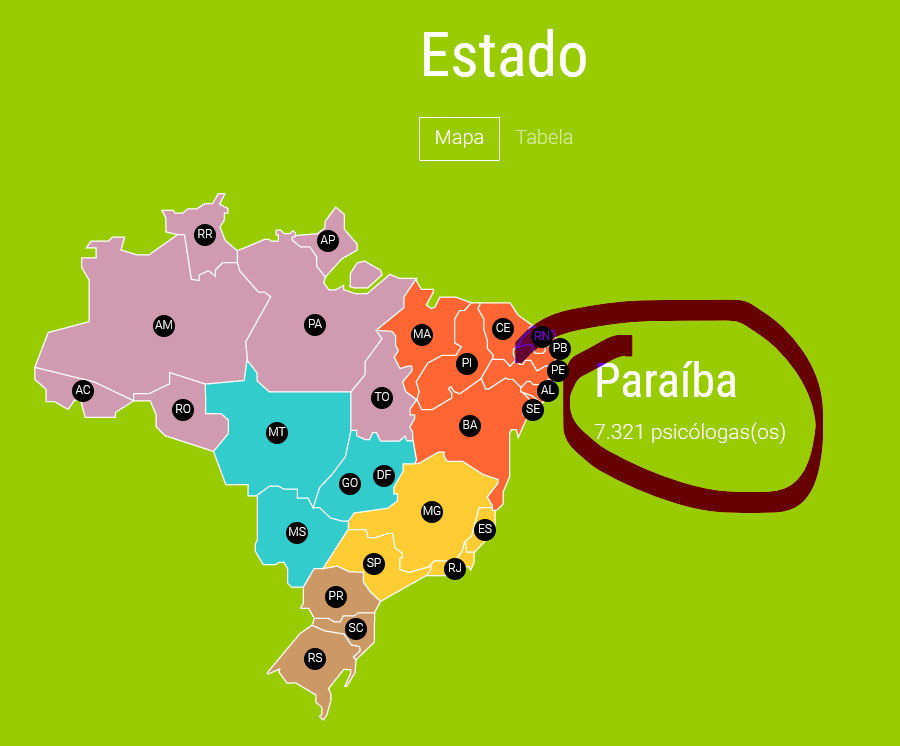
\includegraphics[width=0.5\linewidth]{imagens/numeros-de-psicologia-na-paraiba} 

}

\caption{Número de Psicologos no Brasil e na Paraíba}\label{fig:unnamed-chunk-2}
\end{figure}

\hypertarget{psiquiatria-psicanuxe1lise-e-psicologia}{%
\subsection{Psiquiatria, Psicanálise e Psicologia}\label{psiquiatria-psicanuxe1lise-e-psicologia}}

\begin{quote}
****QUESTÃO DE PROVA****: Psicologia, Psicanálise e Psiquiatria: O que eles apresentam
de semelhança entre si? Quais são suas diferenças?
\end{quote}

\begin{itemize}
\tightlist
\item
  \textbf{Psiquiatria}

  \begin{itemize}
  \tightlist
  \item
    É uma \textbf{especialização da Medicina}
  \item
    É voltada ao \textbf{tratamento do transtorno mental}.
  \end{itemize}
\item
  \textbf{Psicanálise}

  \begin{itemize}
  \tightlist
  \item
    Um ****método de investigação****;
  \item
    Consiste essencialmente em \textbf{evidenciar o significado inconsciente} das \textbf{palavras}, das \textbf{ações} de uma pessoa
  \end{itemize}
\item
  \textbf{Psicologia}

  \begin{itemize}
  \tightlist
  \item
    É a \textbf{ciência} que estuda o \textbf{comportamento} e os \textbf{processos mentais}.
  \end{itemize}
\end{itemize}

\hypertarget{perspectivas-histuxf3ricas}{%
\subsection{Perspectivas Históricas}\label{perspectivas-histuxf3ricas}}

\hypertarget{aristuxf3teles-328-a.c.}{%
\subsubsection{Aristóteles (328 a.C.)}\label{aristuxf3teles-328-a.c.}}

\begin{itemize}
\tightlist
\item
  ``Pai da Psicologia'' séculos antes os primeiros filósofos lidavam com questões relacionadas o comportamento humano
\end{itemize}

\hypertarget{gustav-fechner}{%
\subsubsection{Gustav Fechner}\label{gustav-fechner}}

\begin{figure}

{\centering 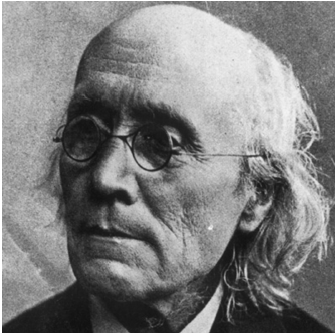
\includegraphics[width=0.5\linewidth]{imagens/GustavFechner} 

}

\caption{Gustav Fechner}\label{fig:unnamed-chunk-3}
\end{figure}

\begin{itemize}
\tightlist
\item
  Relação entre estímulo físico e sensação ( Lei de Weber-Fechner em 1860 ).
\item
  Principal trabalho: Elementos da psicofísica (1860)
\item
  Procedimentos experimentais e matemáticos.
\item
  Questões:

  \begin{itemize}
  \tightlist
  \item
    Quanto deve brilhar uma estrela para ser vista ?
  \item
    Quão alto deve ser um ruído para ser ouvido ?
  \item
    Quão forte deve ser um toque para ser sentido ?
  \end{itemize}
\end{itemize}

\hypertarget{william-james}{%
\subsubsection{William James}\label{william-james}}

\begin{figure}

{\centering 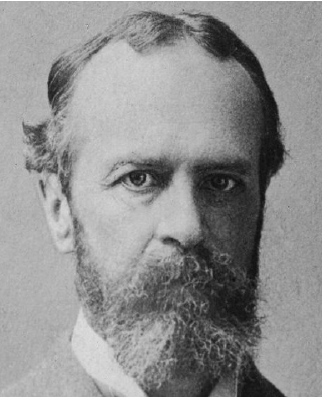
\includegraphics[width=0.5\linewidth]{imagens/WilliamJames} 

}

\caption{William James}\label{fig:unnamed-chunk-4}
\end{figure}

\begin{itemize}
\tightlist
\item
  Formação em fisiologista;
\item
  Laboratório para demonstração dos fatores fisiológicos que influenciam a psicologia;
\item
  Crítica a psicologia Wundtiana
\item
  Consciência:

  \begin{itemize}
  \tightlist
  \item
    Seu funcionamento e como a utilizar para adaptação ao meio
  \item
    Funcionalismo: Em vez de tratar a \textbf{estrutura da mente}, o \textbf{funcionalismo concentrou} se \textbf{no que a mente faz} e em \textbf{como o comportamento funciona}.
  \end{itemize}
\end{itemize}

\hypertarget{wilhelm-wundt}{%
\subsubsection{Wilhelm Wundt}\label{wilhelm-wundt}}

\begin{figure}

{\centering 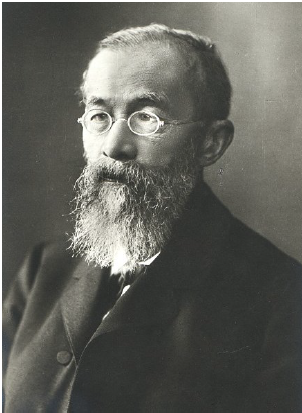
\includegraphics[width=0.5\linewidth]{imagens/WilhelmWundt} 

}

\caption{Wilhelm Wundt}\label{fig:unnamed-chunk-5}
\end{figure}

\begin{itemize}
\tightlist
\item
  \textbf{O primeiro a separar a Psicologa} como parte da Filosofia
\item
  Origem da Psicologia

  \begin{itemize}
  \tightlist
  \item
    1º Laboratório de pesquisa em Psicologia 1879 na Alemanha
  \item
    Os processos elementares da consciência humana
  \end{itemize}
\item
  \textbf{Estruturalismo}: Revelação dos ****componentes fundamentais**** da \textbf{percepção}, da \textbf{consciência}, do \textbf{pensamento}, das \textbf{emoções} e de \textbf{outros tipos de }estados** e \textbf{atividades} mentais**
\item
  \textbf{Introspecção}: Procedimento usado para estudar da mente, no qual se pede aos sujeitos que descrevam detalhadamente o que eles estão sentindo quando são expostos a um estímulo. É uma \textbf{autoanálise} da mente para \textbf{inspecionar} e \textbf{relatar} \textbf{pensamentos} e \textbf{sentimentos} pessoais. (SCHULTZ \& SCHULTZ,2015)
\end{itemize}

\hypertarget{referuxeancias}{%
\paragraph{Referências}\label{referuxeancias}}

SHULTZ, Duane P.; SHULTZ, Sydney Ellen \textbf{História da psicologia moderna} 2014. 10. ed.~São Paulo: Cengage Learning.

\hypertarget{psicologia-do-suxe9culo-xx}{%
\subsection{Psicologia do Século XX}\label{psicologia-do-suxe9culo-xx}}

\begin{figure}

{\centering 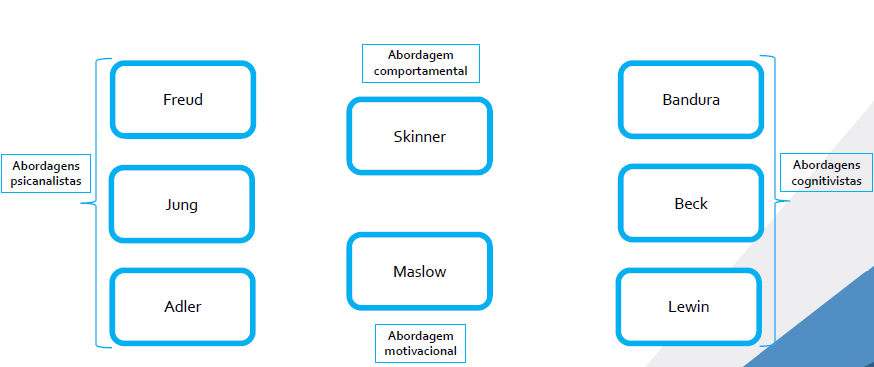
\includegraphics[width=0.8\linewidth]{imagens/psicologos-do-seculo-xx} 

}

\caption{Psicologos do Século XX}\label{fig:unnamed-chunk-6}
\end{figure}

\hypertarget{princuxedpios-guia-da-pesquisa}{%
\subsection{Princípios-guia da Pesquisa}\label{princuxedpios-guia-da-pesquisa}}

Segundo Skinner (1953) apud Davidoff (2001), são apontados seis princípios sobre o que significa \textbf{ciência}:

\begin{itemize}
\tightlist
\item
  \textbf{Precisão}:

  \begin{itemize}
  \tightlist
  \item
    Os psicólogos precisam ser precisos (definir \textbf{especificamente o que procuram faze}r).
  \end{itemize}
\item
  \textbf{Objetividade}

  \begin{itemize}
  \tightlist
  \item
    Tomar medidas que impeçam a influência do \textbf{ponto de vista particular} nos estudos.
  \end{itemize}
\item
  \textbf{Empirismo}

  \begin{itemize}
  \tightlist
  \item
    \textbf{Forma de conhecimento} através da \textbf{observação} \textbf{direta} e \textbf{indireta}.
  \item
    O empirismo consiste em \textbf{uma teoria epistemológica} que indica que \textbf{todo o }conhecimento** é um \textbf{fruto da experiência}**, e por isso, uma consequência dos sentidos. A experiência estabelece o valor, a origem e os limites do conhecimento.
  \end{itemize}
\item
  \textbf{Determinismo}

  \begin{itemize}
  \tightlist
  \item
    Refere-se à crença de que todos os ****eventos** tem \textbf{causas} naturais** (fatores internos e externos).
  \end{itemize}
\item
  \textbf{Parcimônia}

  \begin{itemize}
  \tightlist
  \item
    Um padrão sobre as explicações dos fenômenos, em que a \textbf{preferência se volta para }explicações simples**** que se ajustem aos fatos observados.
  \item
    Não ter pressa em manifestar conclusões que devem ser emitidas com precaução, cuidado e atenção.
  \item
    A palavra também significa ``aquilo que é essencial ou suficiente para suprir determinada necessidade''
  \end{itemize}
\item
  \textbf{Ceticismo}

  \begin{itemize}
  \tightlist
  \item
    Idealmente, os psicólogos são críticos em relação ao seu trabalho e ao de outros pesquisadores.
  \end{itemize}
\end{itemize}

\hypertarget{questuxf5es-que-os-psicuxf3logos-levantam}{%
\subsection{Questões que os psicólogos levantam}\label{questuxf5es-que-os-psicuxf3logos-levantam}}

\hypertarget{slide-metas-de-pesquisa-em-psicologia}{%
\section{Slide ``Metas de Pesquisa em Psicologia''}\label{slide-metas-de-pesquisa-em-psicologia}}

\hypertarget{etapas-de-uma-pesquisa}{%
\subsection{Etapas de uma pesquisa}\label{etapas-de-uma-pesquisa}}

\begin{figure}

{\centering 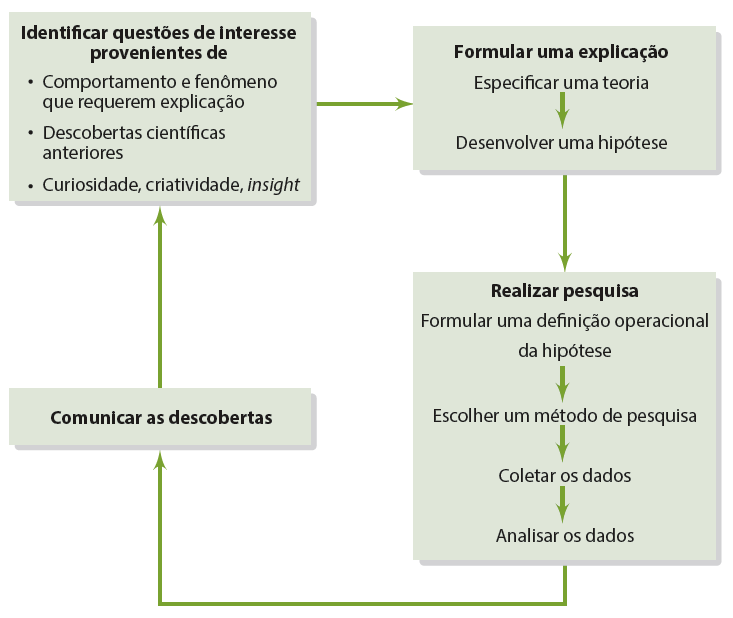
\includegraphics[width=0.8\linewidth]{imagens/o-metodo-cientifico} 

}

\caption{O método científico}\label{fig:unnamed-chunk-8}
\end{figure}

\begin{itemize}
\tightlist
\item
  As visões do senso comum são frequentemente contraditórias;
\item
  Uma das \textbf{PRIMEIRAS MISSÕES} para o campo da psicologia é \textbf{desenvolver suposições sobre o comportamento} e determinar \textbf{quais dessas suposições são }precisas****;
\item
  Todos os cientistas, incluindo os psicólogos, enfrentam o desafio de ****propor questões apropriadas**** e ****respondê-las**** adequadamente utilizando o ****método científico****;
\item
  O ****método científico****, para os psicólogos:

  \begin{itemize}
  \tightlist
  \item
    Abrange o processo de (1) identificar, (2) formular e (3) responder questões para chegar a uma compreensão sobre o mundo;
  \item
    É uma abordagem usada para ****adquirir**** sistematicamente \textbf{conhecimento} e \textbf{compreensão} sobre:

    \begin{enumerate}
    \def\labelenumi{\alph{enumi}.}
    \tightlist
    \item
      o comportamento;
    \item
      outros fenômenos de interesse;
    \end{enumerate}
  \item
    Consiste em ****QUATRO PASSOS**** principais:

    \begin{enumerate}
    \def\labelenumi{\alph{enumi}.}
    \tightlist
    \item
      \textbf{PASSO 1} - Identificar ****questões de interesse**** (O QUE ?);

      \begin{itemize}
      \tightlist
      \item
        Provinientes de \textbf{comportamento} ou \textbf{fenômeno} que requer explicação;
      \item
        Provinientes de \textbf{descobertas científicas anteriores};
      \item
        Provinientes de curiosidade, criatividade, insight, etc.
      \end{itemize}
    \item
      \textbf{PASSO 2} - Formular uma ****explicação**** (POR QUE ?);

      \begin{itemize}
      \tightlist
      \item
        Especificar uma teoria (Necessária no desenvolvimento de uma hipótese)
      \item
        Desenvolver uma hipótese;\\
      \end{itemize}
    \item
      \textbf{PASSO 3} - Realizar pesquisa destinada a ****apoiar**** ou ****refutar**** a explicação \textbf{utilizando um }método**** (COMO ?);
    \item
      Formular uma \textbf{definição operacional} da hipótese;

      \begin{itemize}
      \tightlist
      \item
        A \textbf{definição operacional} é o como (passo a passo) o pesquisador vai colocar em prática o teste da hipótese)
      \end{itemize}
    \item
      Escolher um método de pesquisa;

      \begin{itemize}
      \tightlist
      \item
        Coletar dados;
      \item
        Analisar dados;
      \end{itemize}
    \item
      \textbf{PASSO 4} - ****Comunicar**** descobertas;
    \end{enumerate}
  \end{itemize}
\end{itemize}

\begin{figure}

{\centering 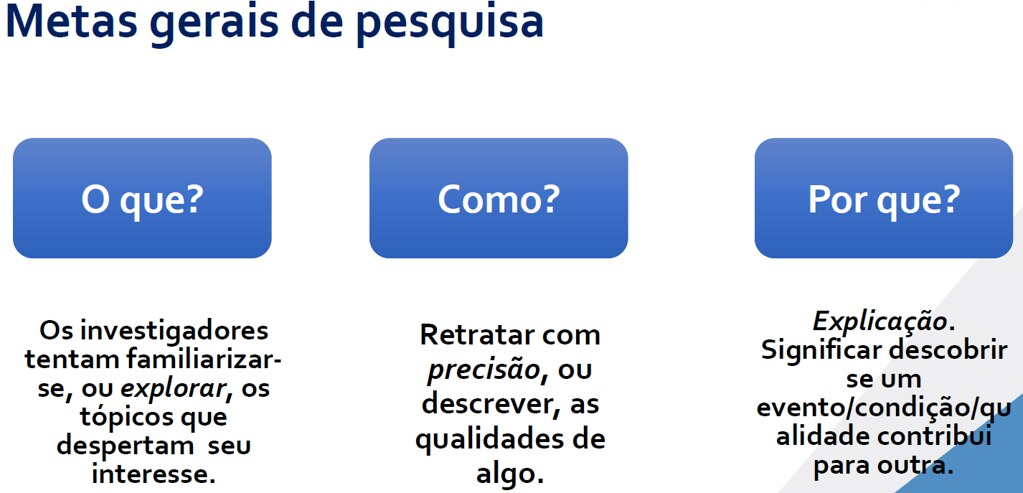
\includegraphics[width=0.8\linewidth]{imagens/slide-2-pagina-4-metas-gerais-de-pesquisa} 

}

\caption{Metas gerais de pesquisa (slide 2 / página 4)}\label{fig:unnamed-chunk-9}
\end{figure}

\hypertarget{muxe9todo-cientuxedfico}{%
\subsection{Método Científico}\label{muxe9todo-cientuxedfico}}

\begin{itemize}
\tightlist
\item
  \textbf{Método Não Experimental ( Pesquisa Descritiva )}

  \begin{itemize}
  \tightlist
  \item
    Pesquisa de Arquivo
  \item
    Observações Diretas

    \begin{itemize}
    \tightlist
    \item
      Observações de Laboratório
    \item
      Observações de Campo
    \end{itemize}
  \item
    Pesquisa de Levantamento - Instrumentos de avaliação

    \begin{itemize}
    \tightlist
    \item
      Questionários
    \item
      Entrevistas
    \item
      Testes psicológicos
    \end{itemize}
  \item
    Estudos de Caso
  \item
    Pesquisa Correlacional
  \end{itemize}
\item
  \textbf{Exemplos:}

  \begin{itemize}
  \tightlist
  \item
    \textbf{Objetivo}: Será que desempenho profissional se relaciona com esperança, otimismo e criatividade?
  \item
    \textbf{Hipótese} :O desempenho profissional correlaciona positivamente com esperança, otimismo e criatividade
  \item
    \textbf{Resultados}: A autoavaliação do \textbf{desempenho profissional} se correlacionou positivamente com afetos \textbf{esperança}, \textbf{otimismo} e \textbf{criatividade}.
  \end{itemize}
\item
  \textbf{Método Experimental}

  \begin{itemize}
  \tightlist
  \item
    Pesquisa Experimental ( Estudo experimental )
  \end{itemize}
\end{itemize}

\hypertarget{muxe9todo-cientuxedfico-muxe9todo-nuxe3o-experimental-pesquisa-descritiva}{%
\subsubsection{Método Científico: Método Não Experimental ( Pesquisa Descritiva )}\label{muxe9todo-cientuxedfico-muxe9todo-nuxe3o-experimental-pesquisa-descritiva}}

Segundo Feldman (2015), é destinada a investigar sistematicamente ****uma pessoa****, ****um grupo**** ou ****padrões de comportamento****.

\hypertarget{pesquisa-de-arquivo}{%
\subparagraph{PESQUISA DE ARQUIVO}\label{pesquisa-de-arquivo}}

Slide 2 - Aula 17.08.2022

Não foi detalhado no slide. A professora fez explicações que estão contidas no item abaixo do livro de Introdução a Psicologia de Feldman (2015)\textsuperscript{1}

\begin{quote}
\begin{quote}
\begin{quote}
\begin{quote}
\begin{quote}
\begin{quote}
ACRESCENTAR LINK PARA SECAO DO RESUMO DOS LIVROS
\end{quote}
\end{quote}
\end{quote}
\end{quote}
\end{quote}
\end{quote}

\hypertarget{observauxe7uxe3o-direta-observauxe7uxe3o-naturalista}{%
\subparagraph{OBSERVAÇÃO DIRETA ( Observação Naturalista )}\label{observauxe7uxe3o-direta-observauxe7uxe3o-naturalista}}

Slide 2 - Aula 17.08.2022

\begin{itemize}
\tightlist
\item
  LABORATÓRIO

  \begin{itemize}
  \tightlist
  \item
    Para observação direta, é a criação em laboratório de um ambiente padrão que estimule o comportamento de interesse e permita a coleta de informações aprimoradas.
  \item
    \textbf{Limitações} da Pesquisa de Laboratório

    \begin{itemize}
    \tightlist
    \item
      Artificialidade;
    \item
      Aplicação das descobertas de laboratório à vida real.
    \end{itemize}
  \end{itemize}
\item
  CAMPO

  \begin{itemize}
  \tightlist
  \item
    Observação naturalista, que implica a observação do comportamento diretamente no seu ambiente natural, sendo mais realista.
  \end{itemize}
\end{itemize}

\begin{quote}
\begin{quote}
\begin{quote}
\begin{quote}
\begin{quote}
\begin{quote}
ACRESCENTAR LINK PARA SECAO DO RESUMO DOS LIVROS
\end{quote}
\end{quote}
\end{quote}
\end{quote}
\end{quote}
\end{quote}

\hypertarget{pesquisa-de-levantamento}{%
\subparagraph{PESQUISA DE LEVANTAMENTO}\label{pesquisa-de-levantamento}}

Slide 2 - Aula 17.08.2022

\begin{itemize}
\tightlist
\item
  QUESTIONÁRIOS

  \begin{itemize}
  \tightlist
  \item
    Perguntas diretas na coleta de informações sobre o pensamento e o comportamento de um número suficiente de indivíduos.
  \end{itemize}
\item
  ENTREVISTAS

  \begin{itemize}
  \tightlist
  \item
    Similar aos questionários. Os autorrelatos são obtidos diretamente (presencial).
  \item
    Elas se dividem em:

    \begin{itemize}
    \tightlist
    \item
      Estruturadas;
    \item
      Abertas; e
    \item
      Semi-estruturadas.
    \end{itemize}
  \end{itemize}
\item
  TESTES PSICOLÓGICOS

  \begin{itemize}
  \tightlist
  \item
    São projetados para medir conceitos que não podem ser observados diretamente: inteligência, melancolia, traços de personalidade, crenças, sentimentos, etc.
  \end{itemize}
\end{itemize}

\begin{figure}

{\centering 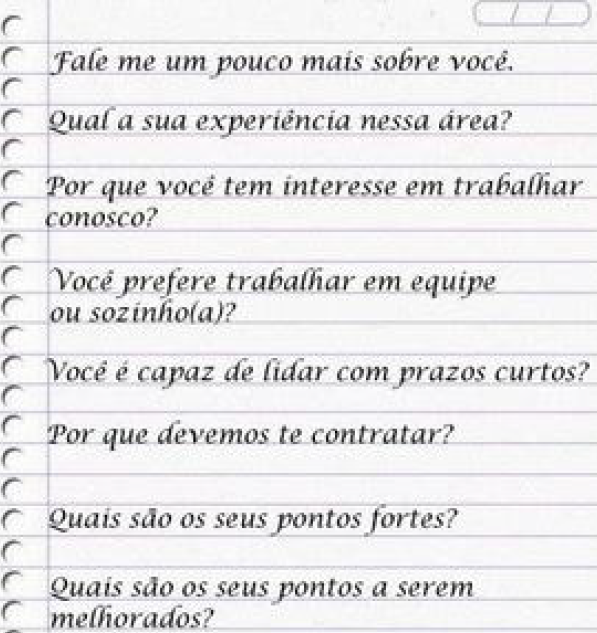
\includegraphics[width=0.5\linewidth]{imagens/entrevista-exemplo1} 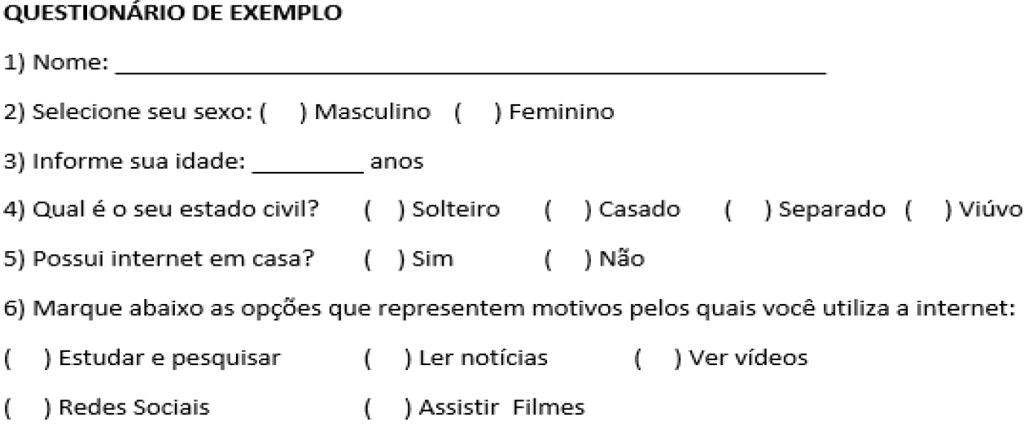
\includegraphics[width=0.5\linewidth]{imagens/entrevista-exemplo2} 

}

\caption{Exemplos de Entrevista}\label{fig:unnamed-chunk-10}
\end{figure}

\begin{figure}

{\centering 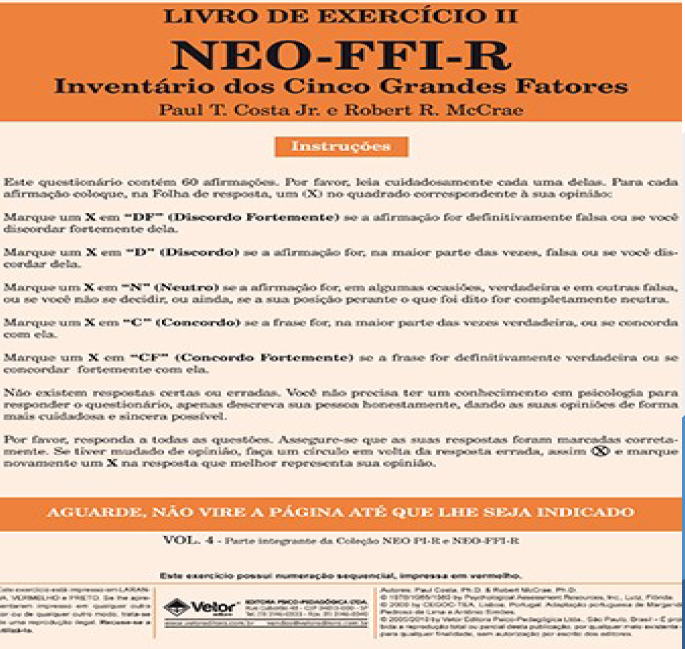
\includegraphics[width=0.8\linewidth]{imagens/teste-neo-pi-r} 

}

\caption{Teste NEO PI-R}\label{fig:unnamed-chunk-11}
\end{figure}

Modelo que seja capaz de identificar as dimensões básicas da personalidade, que possa ser compreendido e reconhecido nas diferentes culturas e nacionalidades

\begin{figure}

{\centering 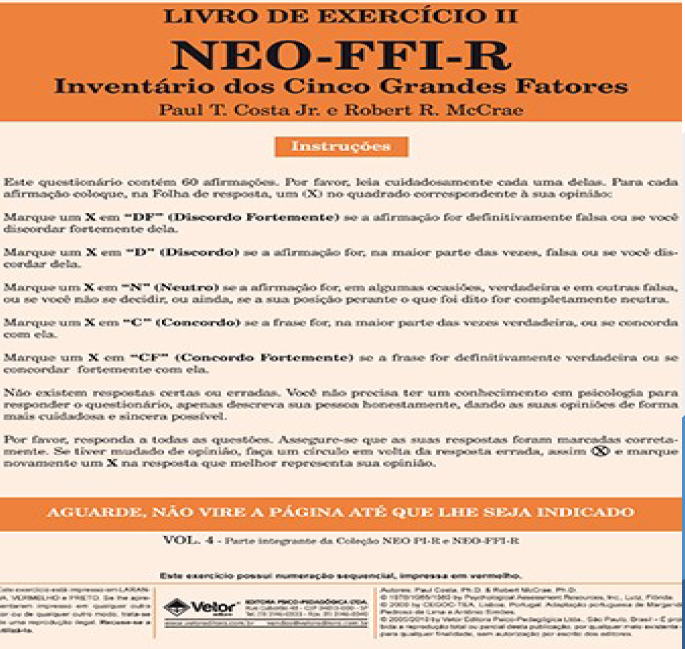
\includegraphics[width=0.8\linewidth]{imagens/teste-neo-pi-r} 

}

\caption{Teste NEO PI-R}\label{fig:unnamed-chunk-12}
\end{figure}

O Neo-Pi-R -- ou Inventário de Personalidade NEO PI Revisado -- é um teste de personalidade adulta reconhecido internacionalmente por seu elevado rigor na avaliação e construção de resultados. Ele conta com uma base teórica que considera cinco grandes fatores para compreender os contornos da subjetividade de um indivíduo.

Ainda que hoje o Neo-Pi-R seja bem aceito e largamente utilizado, é importante lembrar que avaliar personalidades não é uma tarefa simples. Precisamos ter cuidado para não tomar como verdade suposições generalistas que pouco condizem com a realidade. Além disso, existe o desafio de criar definições básicas e claras o suficiente para que sejam compreendidas por diferentes culturas e nacionalidades.

Hoje, compreendemos a teoria dos cinco grandes fatores como um das mais eficientes e universalmente compreensíveis. Em especial, o Inventário de Personalidade NEO PI Revisado surge como consenso de modelo mais adequado para avaliar personalidades dentro de diferentes culturas. Por isso, ele tem sido muito utilizado nas últimas décadas.

\begin{figure}

{\centering 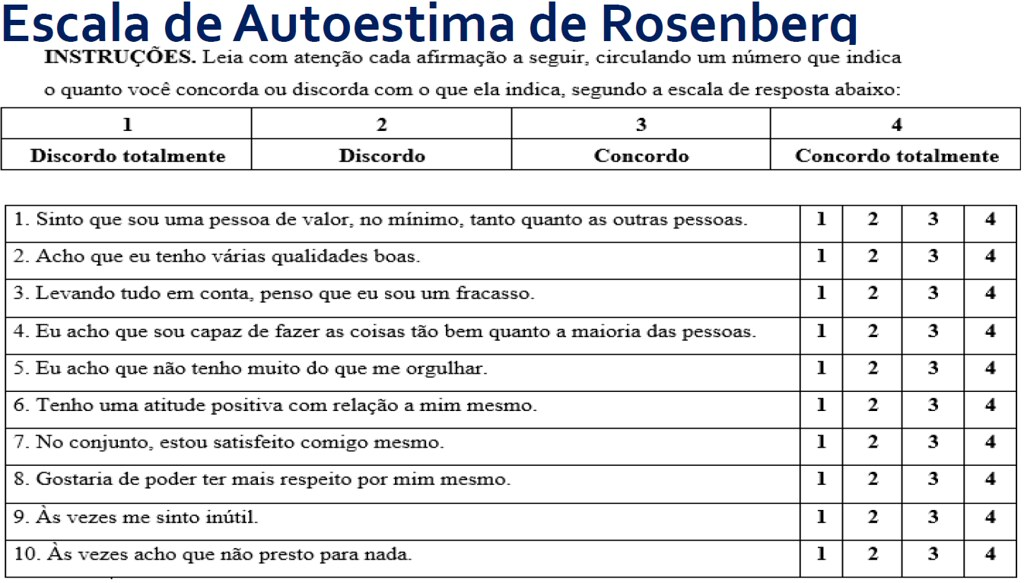
\includegraphics[width=0.8\linewidth]{imagens/teste-autoestima-rosenberg} 

}

\caption{Teste de Autoestima de Rosenberg}\label{fig:unnamed-chunk-13}
\end{figure}

Desenvolvida pelo sociólogo Dr.~Morris Rosenberg, a escala de Rosenberg é uma medida de autoestima amplamente utilizada em pesquisas de ciências sociais. Ele usa uma escala de 0 a 30, em que uma pontuação inferior a 15 pode indicar baixa autoestima problemática. A escala consiste em dez afirmações que você poderia aplicar a você e que deve avaliar o quanto concorda com cada uma. Os itens devem ser respondidos rapidamente, sem pensar demais, sua primeira inclinação é o que você deve anotar.

\hypertarget{estudo-de-caso}{%
\subparagraph{ESTUDO DE CASO}\label{estudo-de-caso}}

Slide 2 - Aula 17.08.2022

\begin{itemize}
\tightlist
\item
  Baseiam se na coleta de informações detalhadas sobre um mesmo indivíduo ou grupo, durante um longo período
\end{itemize}

\begin{figure}

{\centering 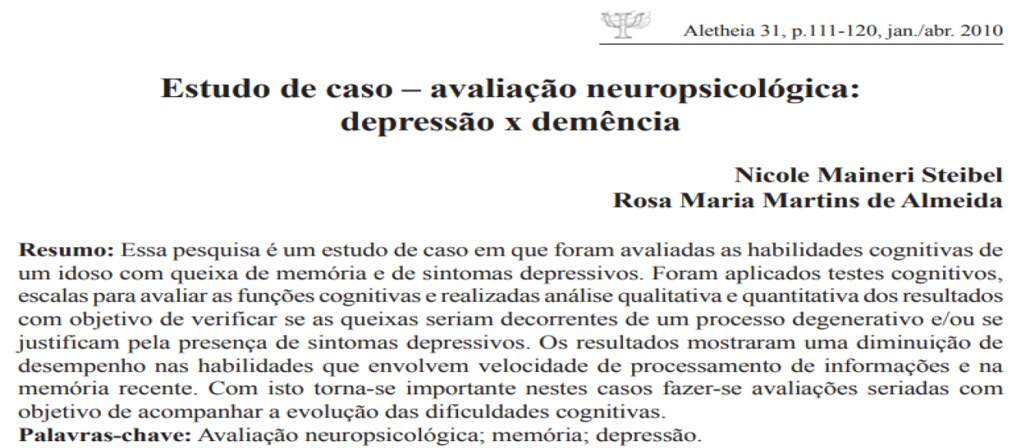
\includegraphics[width=0.8\linewidth]{imagens/estudo-de-caso-individual} 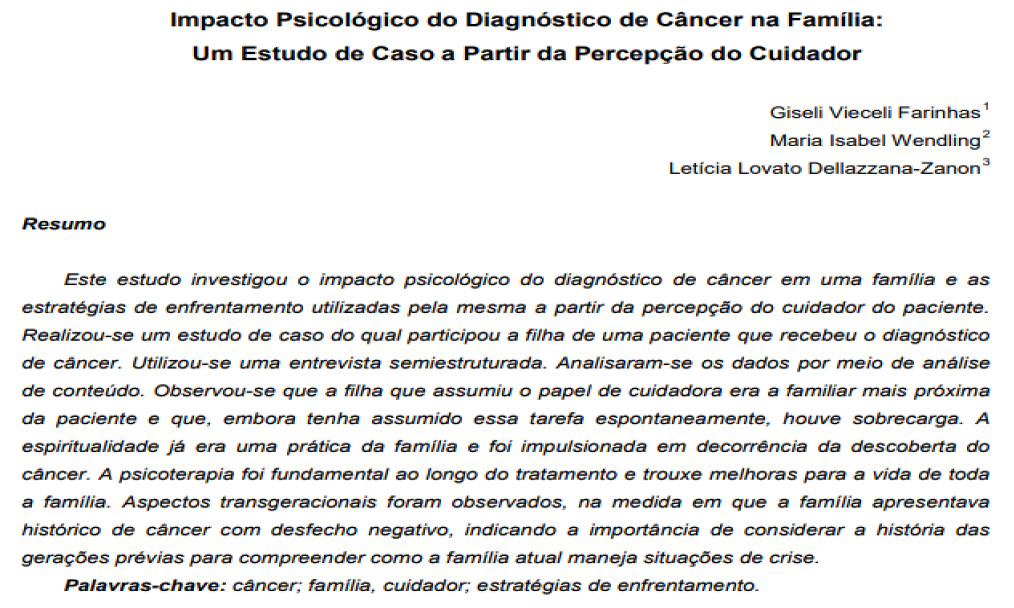
\includegraphics[width=0.8\linewidth]{imagens/estudo-de-caso-pequeno-grupo} 

}

\caption{Estudo de Caso Individual e Estudo de Caso de um Pequeno Grupo}\label{fig:unnamed-chunk-14}
\end{figure}

\begin{quote}
\begin{quote}
\begin{quote}
\begin{quote}
\begin{quote}
\begin{quote}
ACRESCENTAR LINK PARA SECAO DO RESUMO DOS LIVROS
\end{quote}
\end{quote}
\end{quote}
\end{quote}
\end{quote}
\end{quote}

\hypertarget{pesquisa-correlacional}{%
\subparagraph{PESQUISA CORRELACIONAL}\label{pesquisa-correlacional}}

Slide 2 - Aula 17.08.2022

\begin{quote}
****ATENÇÃO PARA PROVA:**** \textbf{CORRELAÇÕES NÃO SIGNIFICAM CAUSA !!!}
\end{quote}

\begin{itemize}
\tightlist
\item
  A ****premissa básica**** é de que \textbf{duas variáveis} estão relacionadas.
\item
  Variam em:

  \begin{itemize}
  \tightlist
  \item
    Intensidade (fraco, moderado ou forte)
  \item
    Direção (positivo ou negativo)
  \end{itemize}
\item
  \textbf{VARIÁVEL}: É aquilo que varia. É fenômeno que assume mais de um valor.
\end{itemize}

Exemplo

\begin{itemize}
\tightlist
\item
  \textbf{Objetivo}: Será que \textbf{desempenho profissional} se relaciona com \textbf{esperança}, \textbf{otimismo} e \textbf{criatividade} ?
\item
  \textbf{Hipótese}: O desempenho profissional correlaciona positivamente com esperança, otimismo e criatividade
\item
  \textbf{Resultados}: A autoavaliação do desempenho profissional se correlacionou positivamente com afetos esperança, otimismo e criatividade
\end{itemize}

\begin{figure}

{\centering 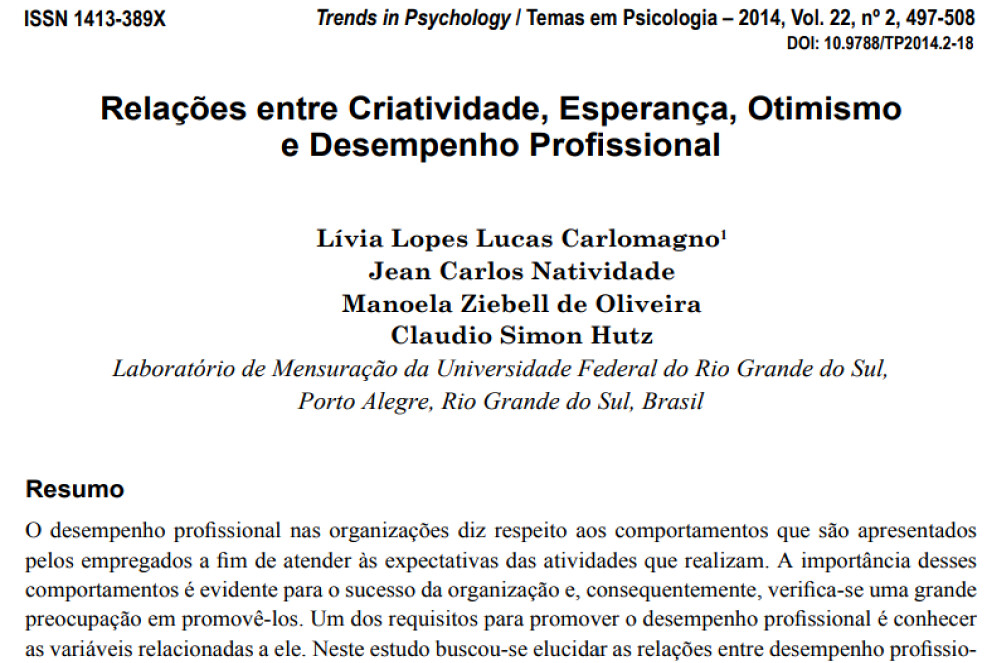
\includegraphics[width=0.8\linewidth]{imagens/exemplo-pesquisa-correlacional} 

}

\caption{Exemplo de pesquisa correlacional}\label{fig:unnamed-chunk-15}
\end{figure}

\begin{quote}
\begin{quote}
\begin{quote}
\begin{quote}
\begin{quote}
\begin{quote}
ACRESCENTAR LINK PARA SECAO DO RESUMO DOS LIVROS
\end{quote}
\end{quote}
\end{quote}
\end{quote}
\end{quote}
\end{quote}

\hypertarget{slide-psicanuxe1lise-x-behaviorismo}{%
\section{Slide ``Psicanálise x Behaviorismo''}\label{slide-psicanuxe1lise-x-behaviorismo}}

\begin{itemize}
\tightlist
\item
  Embora os slides estejam disponíveis, ainda não tivemos tempo para elaborar o resumo deles. Vou disponibilizar em breve.
\end{itemize}

\hypertarget{slide-gestalt-x-cogniuxe7uxe3o}{%
\section{Slide ``Gestalt x Cognição''}\label{slide-gestalt-x-cogniuxe7uxe3o}}

\begin{itemize}
\tightlist
\item
  Embora os slides estejam disponíveis, ainda não tivemos tempo para elaborar o resumo deles. Vou disponibilizar em breve.
\end{itemize}

\hypertarget{slide-abordagem-humanista}{%
\section{Slide ``Abordagem Humanista''}\label{slide-abordagem-humanista}}

\begin{itemize}
\tightlist
\item
  Embora os slides estejam disponíveis, ainda não tivemos tempo para elaborar o resumo deles. Vou disponibilizar em breve.
\end{itemize}

\hypertarget{referuxeancias-bibliogruxe1ficas-1}{%
\section{Referências Bibliográficas}\label{referuxeancias-bibliogruxe1ficas-1}}

FELDMAN, Robert S. Pesquisa em Psicologia. \emph{In:} Feldman, Robert S. \textbf{Introdução à Psicologia}. 10. ed.~Porto Alegre: AMGH Editora, 2015, p.~26-39

RIBEIRO, Maria Gabriela Costa. \textbf{Slide Introdução à Psicologia}. Introdução à Psicologia. Notas de aula, Faculdade Três Marias, Paraíba 2022.

RIBEIRO, Maria Gabriela Costa. \textbf{Slide Metas de Pesquisa em Psicologia}. Introdução à Psicologia. Notas de aula, Faculdade Três Marias, Paraíba 2022.

RIBEIRO, Maria Gabriela Costa Ribeiro. \textbf{Slide Psicanálise x Behaviorismo}. Introdução à Psicologia, Faculdade Três Marias, Paraíba 2022

RIBEIRO, Maria Gabriela Costa Ribeiro. \textbf{Slide Gestalt x Cognição}. Introdução à Psicologia, Faculdade Três Marias, Paraíba 2022

RIBEIRO, Maria Gabriela Costa Ribeiro. \textbf{Slide Abordagem Humanista}. Introdução à Psicologia, Faculdade Três Marias, Paraíba 2022

SHULTZ, Duane P.; SHULTZ, Sydney Ellen História da psicologia moderna 2014. 10. ed.~São Paulo: Cengage Learning.

\hypertarget{p1---histuxf3ria-da-psicologia}{%
\chapter{P1 - História da Psicologia}\label{p1---histuxf3ria-da-psicologia}}

Neste capítulo estarão contidos os resumos dos slides da disciplina História da Psicologia.

Em breve\ldots{}

\hypertarget{p1---leitura-e-produuxe7uxe3o-textual}{%
\chapter{P1 - Leitura e Produção Textual}\label{p1---leitura-e-produuxe7uxe3o-textual}}

Neste capítulo estarão contidos os resumos dos slides da disciplina Leitura e Produção Textual.

Em breve\ldots{}

\hypertarget{p1---metodologia-cientuxedfica}{%
\chapter{P1 - Metodologia Científica}\label{p1---metodologia-cientuxedfica}}

Neste capítulo estarão contidos os resumos dos slides da disciplina Metodologia Científica.

\hypertarget{slides-da-aula-06---normas-abnt-para-elaborauxe7uxe3o-de-trabalhos-cientuxedficos}{%
\section{Slides da Aula 06 - ``Normas ABNT para Elaboração de Trabalhos Científicos''}\label{slides-da-aula-06---normas-abnt-para-elaborauxe7uxe3o-de-trabalhos-cientuxedficos}}

\hypertarget{trabalhos-acaduxeamicos}{%
\subsection{Trabalhos Acadêmicos}\label{trabalhos-acaduxeamicos}}

\hypertarget{definiuxe7uxf5es}{%
\subsubsection{Definições}\label{definiuxe7uxf5es}}

\begin{itemize}
\tightlist
\item
  \textbf{MONOGRAFIA}:

  \begin{itemize}
  \tightlist
  \item
    Término do curso de graduação: os estudantes têm o compromisso de elaborar um trabalho mais aprofundado
  \item
    É a exposição exaustiva de um problema ou assunto específico, investigado cientificamente.
  \item
    É elaborada sob coordenação de um(a) orientador(a).
  \item
    Monografia de graduação: objetiva a obtenção do grau de bacharel, licenciado ou tecnólogo
  \item
    Monografia de especialização: objetiva a obtenção do grau de especialista
  \end{itemize}
\item
  \textbf{DISSERTAÇÃO DE MESTRADO}

  \begin{itemize}
  \tightlist
  \item
    Dissertação um tipo de trabalho científico apresentado ao final do curso de pós-graduação, visando obter o título de mestre/mestra.
  \item
    Situa-se entre a monografia de graduação e a tese de doutorado - aborda temas em maior extensão e profundidade do que a primeira e é fruto de reflexão e de rigor científico, próprio da tese de doutorado, mas sendo ainda um treinamento ou iniciação à investigação
  \end{itemize}
\item
  \textbf{TESE DE DOUTORADO}

  \begin{itemize}
  \tightlist
  \item
    Trabalho científico que apresenta o resultado de um estudo científico ou uma pesquisa experimental de tema específico e bem delimitado.
  \item
    Deve ser elaborada com base em investigação original, constituindo-se em real contribuição para a especialidade em questão
  \end{itemize}
\end{itemize}

\hypertarget{regras-gerais-de-formatauxe7uxe3o}{%
\subsubsection{Regras Gerais de Formatação}\label{regras-gerais-de-formatauxe7uxe3o}}

\begin{longtable}[]{@{}
  >{\raggedright\arraybackslash}p{(\columnwidth - 2\tabcolsep) * \real{0.5000}}
  >{\raggedright\arraybackslash}p{(\columnwidth - 2\tabcolsep) * \real{0.5000}}@{}}
\toprule()
\begin{minipage}[b]{\linewidth}\raggedright
Elemento
\end{minipage} & \begin{minipage}[b]{\linewidth}\raggedright
Regra de Formatação
\end{minipage} \\
\midrule()
\endhead
\textbf{Papel} & Papel branco, formato A4 (21 cm x 29,7 cm), na posição retrato. \\
\textbf{Fonte} & - Arial ou Times New Roman, simples Tamanho 12 para texto e títulos- Cor preta para o texto- Tamanho de fonte 10 para:* citações com mais de três linhas* notas de rodapé* paginação* legendas das ilustrações; * tabelas \\
\textbf{Margens} & - Margem esquerda e superior de 3 cm;- Margem direita e inferior de 2 cm-Justificado \\
\textbf{Espaçamento} & - 1,5 entre linhas:* Para o texto- Simples:* Para Citações diretas de mais de 3 linhas- notas de rodapé- legendas das ilustrações e das tabelas \\
\textbf{Paginação} & - A numeração é colocada a partir da primeira folha da parte textual- Numeração deve ser colocada no anto superior direito \\
\bottomrule()
\end{longtable}

\begin{figure}

{\centering 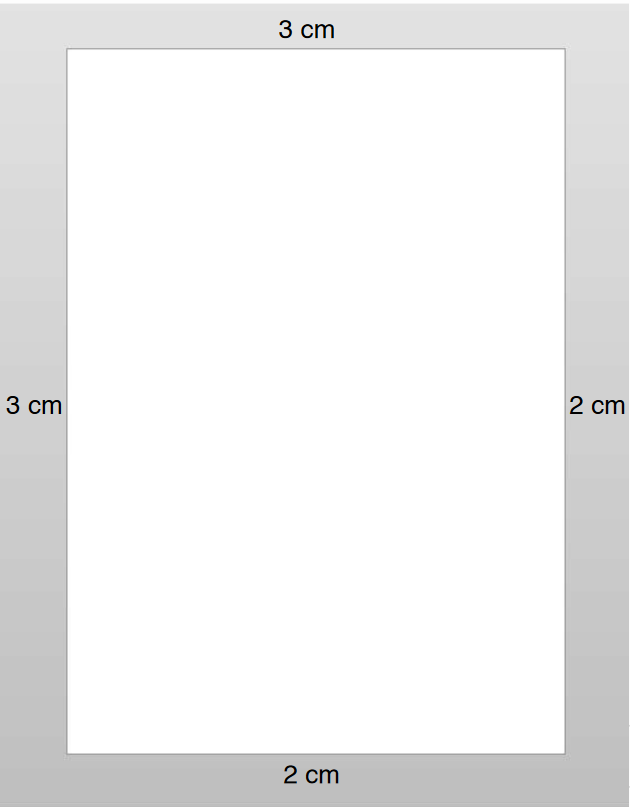
\includegraphics[width=0.8\linewidth]{imagens/exemplo-formatacao-slides-pagina} 

}

\caption{Exemplo de formatação das margens de uma página}\label{fig:unnamed-chunk-16}
\end{figure}

\hypertarget{tuxedtulos-das-seuxe7uxf5es-do-documento}{%
\subsubsection{Títulos das Seções do Documento}\label{tuxedtulos-das-seuxe7uxf5es-do-documento}}

\begin{itemize}
\tightlist
\item
  \textbf{Títulos com indicativo numérico}:

  \begin{itemize}
  \tightlist
  \item
    Alinhados à margem esquerda; e
  \item
    Devem ser precedidos por seu indicativo em algarismos arábicos (não se deve utilizar algarismos romanos) e dele separado por apenas um espaço.
  \end{itemize}
\item
  \textbf{Destacam-se gradativamente}

  \begin{itemize}
  \tightlist
  \item
    Os títulos das seções, utilizando-se os recursos de negrito, itálico, grifo, maiúsculas e versal (no Word, versalete), no texto e de forma idêntica, no sumário.
  \end{itemize}
\end{itemize}

\begin{figure}

{\centering 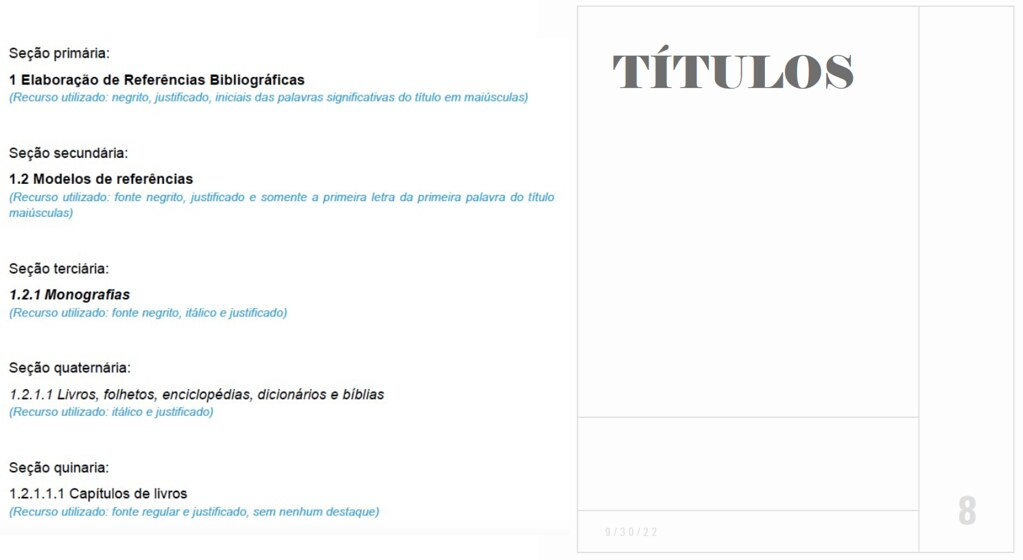
\includegraphics[width=0.8\linewidth]{imagens/titulos-secoes-documentos} 

}

\caption{Títulos das Seções do Documento}\label{fig:unnamed-chunk-17}
\end{figure}

\hypertarget{estrutura-geral-do-trabalho-acaduxeamico}{%
\subsubsection{Estrutura Geral do Trabalho Acadêmico}\label{estrutura-geral-do-trabalho-acaduxeamico}}

\begin{longtable}[]{@{}
  >{\raggedright\arraybackslash}p{(\columnwidth - 4\tabcolsep) * \real{0.3333}}
  >{\raggedright\arraybackslash}p{(\columnwidth - 4\tabcolsep) * \real{0.3333}}
  >{\raggedright\arraybackslash}p{(\columnwidth - 4\tabcolsep) * \real{0.3333}}@{}}
\toprule()
\begin{minipage}[b]{\linewidth}\raggedright
Elemento
\end{minipage} & \begin{minipage}[b]{\linewidth}\raggedright
Regra de Formatação
\end{minipage} & \begin{minipage}[b]{\linewidth}\raggedright
\end{minipage} \\
\midrule()
\endhead
\textbf{Pré-texto} & - Capa- Folha de Rosto- Ficha Catalográfica- Dedicatória- Agradecimentos- Resumo & Abstract- Keywords- Sumário- Lista de Figuras- Lista de Tabelas- Lista de Abreviações- Apresentação \\
\textbf{Texto} & Introdução- Objetivos- Justificativa- Corpo do Trabalho ou Desenvolvimento / Método- Cronograma- Orçamento- Resultados- Conclusões & \\
\textbf{Pós-Texto} & Referências- Anexos- Índice Remissivo- Glossário & \\
\bottomrule()
\end{longtable}

\hypertarget{citauxe7uxf5es}{%
\subsubsection{Citações}\label{citauxe7uxf5es}}

\begin{itemize}
\tightlist
\item
  Citação é a menção, no texto, de informação extraída de outra fonte;
\item
  Todas as citações do texto devem constar nas Referências;
\item
  Todos os documentos relacionados nas Referências devem ser citados no texto;
\item
  Sistema de chamada autor-data entre parênteses: p.~ex.(LEAL, 2022)
\item
  \textbf{Tipos de citação}:

  \begin{itemize}
  \tightlist
  \item
    \textbf{citação direta}: transcrição textual literal de parte da obra do autor consultado;
  \item
    \textbf{citação indireta}: texto escrito baseado na obra do autor consultado;
  \item
    \textbf{citação de citação}: texto escrito em que não se teve acesso ao original.
  \end{itemize}
\end{itemize}

\hypertarget{citauxe7uxe3o-direta}{%
\subsubsection{CITAÇÃO DIRETA}\label{citauxe7uxe3o-direta}}

\hypertarget{atuxe9-3-linhas}{%
\paragraph{ATÉ 3 LINHAS}\label{atuxe9-3-linhas}}

\begin{itemize}
\tightlist
\item
  As citações diretas de \textbf{até três linhas} devem estar contidas entre aspas duplas.
\item
  É obrigatória a menção da paginação de onde tal trecho foi extraído.
\end{itemize}

\hypertarget{mais-de-3-linhas}{%
\subsubsection{MAIS DE 3 LINHAS}\label{mais-de-3-linhas}}

\begin{itemize}
\tightlist
\item
  As citações diretas, no texto, de \textbf{mais de três linhas} devem ser destacadas com recuo de 4 cm da margem esquerda, com Letra menor que a do texto, espaçamento simples e sem aspas.
\item
  É obrigatória a menção da paginação de onde tal trecho foi extraído.
\end{itemize}

\hypertarget{citauxe7uxe3o-indireta}{%
\subsubsection{CITAÇÃO INDIRETA}\label{citauxe7uxe3o-indireta}}

\begin{itemize}
\tightlist
\item
  Transcrição de pensamentos e conceitos do autor consultado, porém descritos com as próprias palavras de quem está escrevendo.
\end{itemize}

\hypertarget{citauxe7uxe3o-de-citauxe7uxe3o}{%
\subsubsection{CITAÇÃO DE CITAÇÃO}\label{citauxe7uxe3o-de-citauxe7uxe3o}}

\begin{itemize}
\tightlist
\item
  Transcrição direta ou indireta de uma obra citada por outro autor, ou seja, a qual não se teve
  acesso.
\item
  Indicar o sobrenome do(s) autor(es) do documento não consultado, seguido da data, da
  expressão latina apud (significa citado por) e do sobrenome do(s) autor(es) do documento
  consultado, data e página.
\item
  OBSERVAÇÃO: Nas REFERÊNCIAS é listada apenas a obra a qual se teve acesso
\end{itemize}

\hypertarget{elementos-essenciais}{%
\subsubsection{ELEMENTOS ESSENCIAIS}\label{elementos-essenciais}}

\hypertarget{como-citar-os-autors-da-informauxe7uxe3o}{%
\paragraph{COMO CITAR O(S) AUTOR(S) DA INFORMAÇÃO}\label{como-citar-os-autors-da-informauxe7uxe3o}}

\hypertarget{um-autor}{%
\subparagraph{Um Autor}\label{um-autor}}

\hypertarget{dois-autores}{%
\subparagraph{Dois Autores}\label{dois-autores}}

\hypertarget{truxeas-autores}{%
\subparagraph{Três Autores}\label{truxeas-autores}}

\hypertarget{mais-que-truxeas-autores}{%
\subparagraph{Mais que Três Autores}\label{mais-que-truxeas-autores}}

\hypertarget{autoria-institucional}{%
\subparagraph{Autoria Institucional}\label{autoria-institucional}}

\hypertarget{no-caso-de-leis-decretos-e-outras-normas}{%
\subparagraph{No caso de Leis, Decretos e Outras Normas}\label{no-caso-de-leis-decretos-e-outras-normas}}

\begin{itemize}
\tightlist
\item
\end{itemize}

  \bibliography{referencias.bib,packages.bib}

\end{document}
